\subsection{Internet Exchange Points (IXPs)}

As part of the decommissioning of the \ac{NSFNET}
in the early-mid 1990s, four \acp{NAP} were created, each operated by
a large American telephone company (MCI, Sprint, PacBell, Ameritech)
to help ensure that the fledgeling commercial Internet did not suffer
a
partition~\cite{hayes1997computing,Ager:2012:ALE:2342356.2342393}. Being
operated by vested interests, the barriers to participation at
the \acp{NAP} were high in terms of cost and equipment. As an
alternative, \acp{IXP} began to appear in carrier-neutral
facilities. The networking community recognised that mutual
interconnections were desireable and that the function of
the \acp{NAP} was a necessary one, but that they ought not to be
operated by carriers because of the conflicts of interest that
inevitably arose. There are now several hundred such \acp{IXP} around
the world.

The role of an \ac{IXP} is primarily economic: if
you have $n$ networks that should be connected together, that is
$\frac{n^2}{2}$ circuits that have to be organised between them,
possibly across many sites. Instead, if these networks agree to meet
at a single place, only $n$ such circuits need to be organised
provided that the central place has some sort of neutral, automatic
multipoint to multipoint switching arrangement. This arrangement is
called an \ac{IXP} and any network present there is free to make
arrangements with any other. To avoid the kinds of conflicts of
interest mentioned above, \acp{IXP} are typically organised as a not
for profit entity, and treated as a cost-centre by its members.

This model of multilateral public peering leads to a very high
density of interconnection and traffic flux across the exchange that
in some cases is comparable in magnitude to the largest global
service providers~\cite{Ager:2012:ALE:2342356.2342393}. This
observation is the first indication that such a topology might be
useful for bringing together several remote networks in order that
this increased density of interconnection can be used to pool traffic
to make collective use of expensive resources such as long-distance
circuits. There are some important differences between the environment
of typical \acp{IXP} and that on the West Coast of Scotland:
\begin{inparaenum}[(i)]
  \item there are no data centres there, carrier-neutral or otherwise;
  \item due to geography there is no single place where all of the
    networks could meet.
\end{inparaenum}



\subsection{Motivating Environment}
The Scottish Highlands and Islands consist of mountainous terrain
stretching 400km North to South consisting of islands in the West
together with deep lochs and glens penetrating the mainland to the
East.  The economy was traditionally maritime, and nearly all
habitation is at sea level or in the glens.

Until recently there was little fibre in the region.  Many exchanges
were served by microwave links. That has started to change, but the
main problem remains that the fibre reaches only to exchanges; and
fibre-based services are available at only a few of them.  Many
communities rely on copper connections to those exchanges in excess of
5km, and there is little prospect of replacing that copper.  In the
medium term future local wireless distribution offers the only
feasible technology for adequate bandwidth and quality of
service\footnote{There is often no mobile reception, and some sites
  cannot "see" satellites.}.

Starting in 2008, the Tegola project~\cite{tegola} started to
experiment with technology that would enable communities to build
their own wireless distribution networks.  This included electrical
and mechanical infrastructure as well as wireless equipment.  It
rapidly became clear that volunteer communities or small businesses
could construct and maintain these networks at a small fraction of the
cost that a centralized organizaton would charge for a number of
reasons: first, the cost and time of travel to service the relays in
remote areas is infinitessimal compared with the cost of a helicopter;
second site licences and wayleaves can usually be negotiated for free
by lightweight agreements; third, we have developed basic technology
(Fig. \ref{fig:mhialairigh}) for robust, inexpensive relay
construction that works well in the mountainous terrain in which the
project operates\footnote{See \url{www.tegola.org.uk}}.

The ideas were taken up by a number of communities across Scotland
including those around the Tegola project shown in Figure
~\ref{fig:whixmap}, which extend over 100km of the coastline. A
typical community would have a local distribution network and
point-to-point links, often in excess of 20km, connected to a
(possibly bonded) set of ADSL lines somewhere near a telephone
exchange. This was far from ideal, but it was the only affordable
source of backhaul. Although the communities shared their expertise
and sometimes their infrastructure, they operated independently.

%% figure as opposed to figure* just in interests of space
%%Thanks
\begin{figure}[h]
\centering
 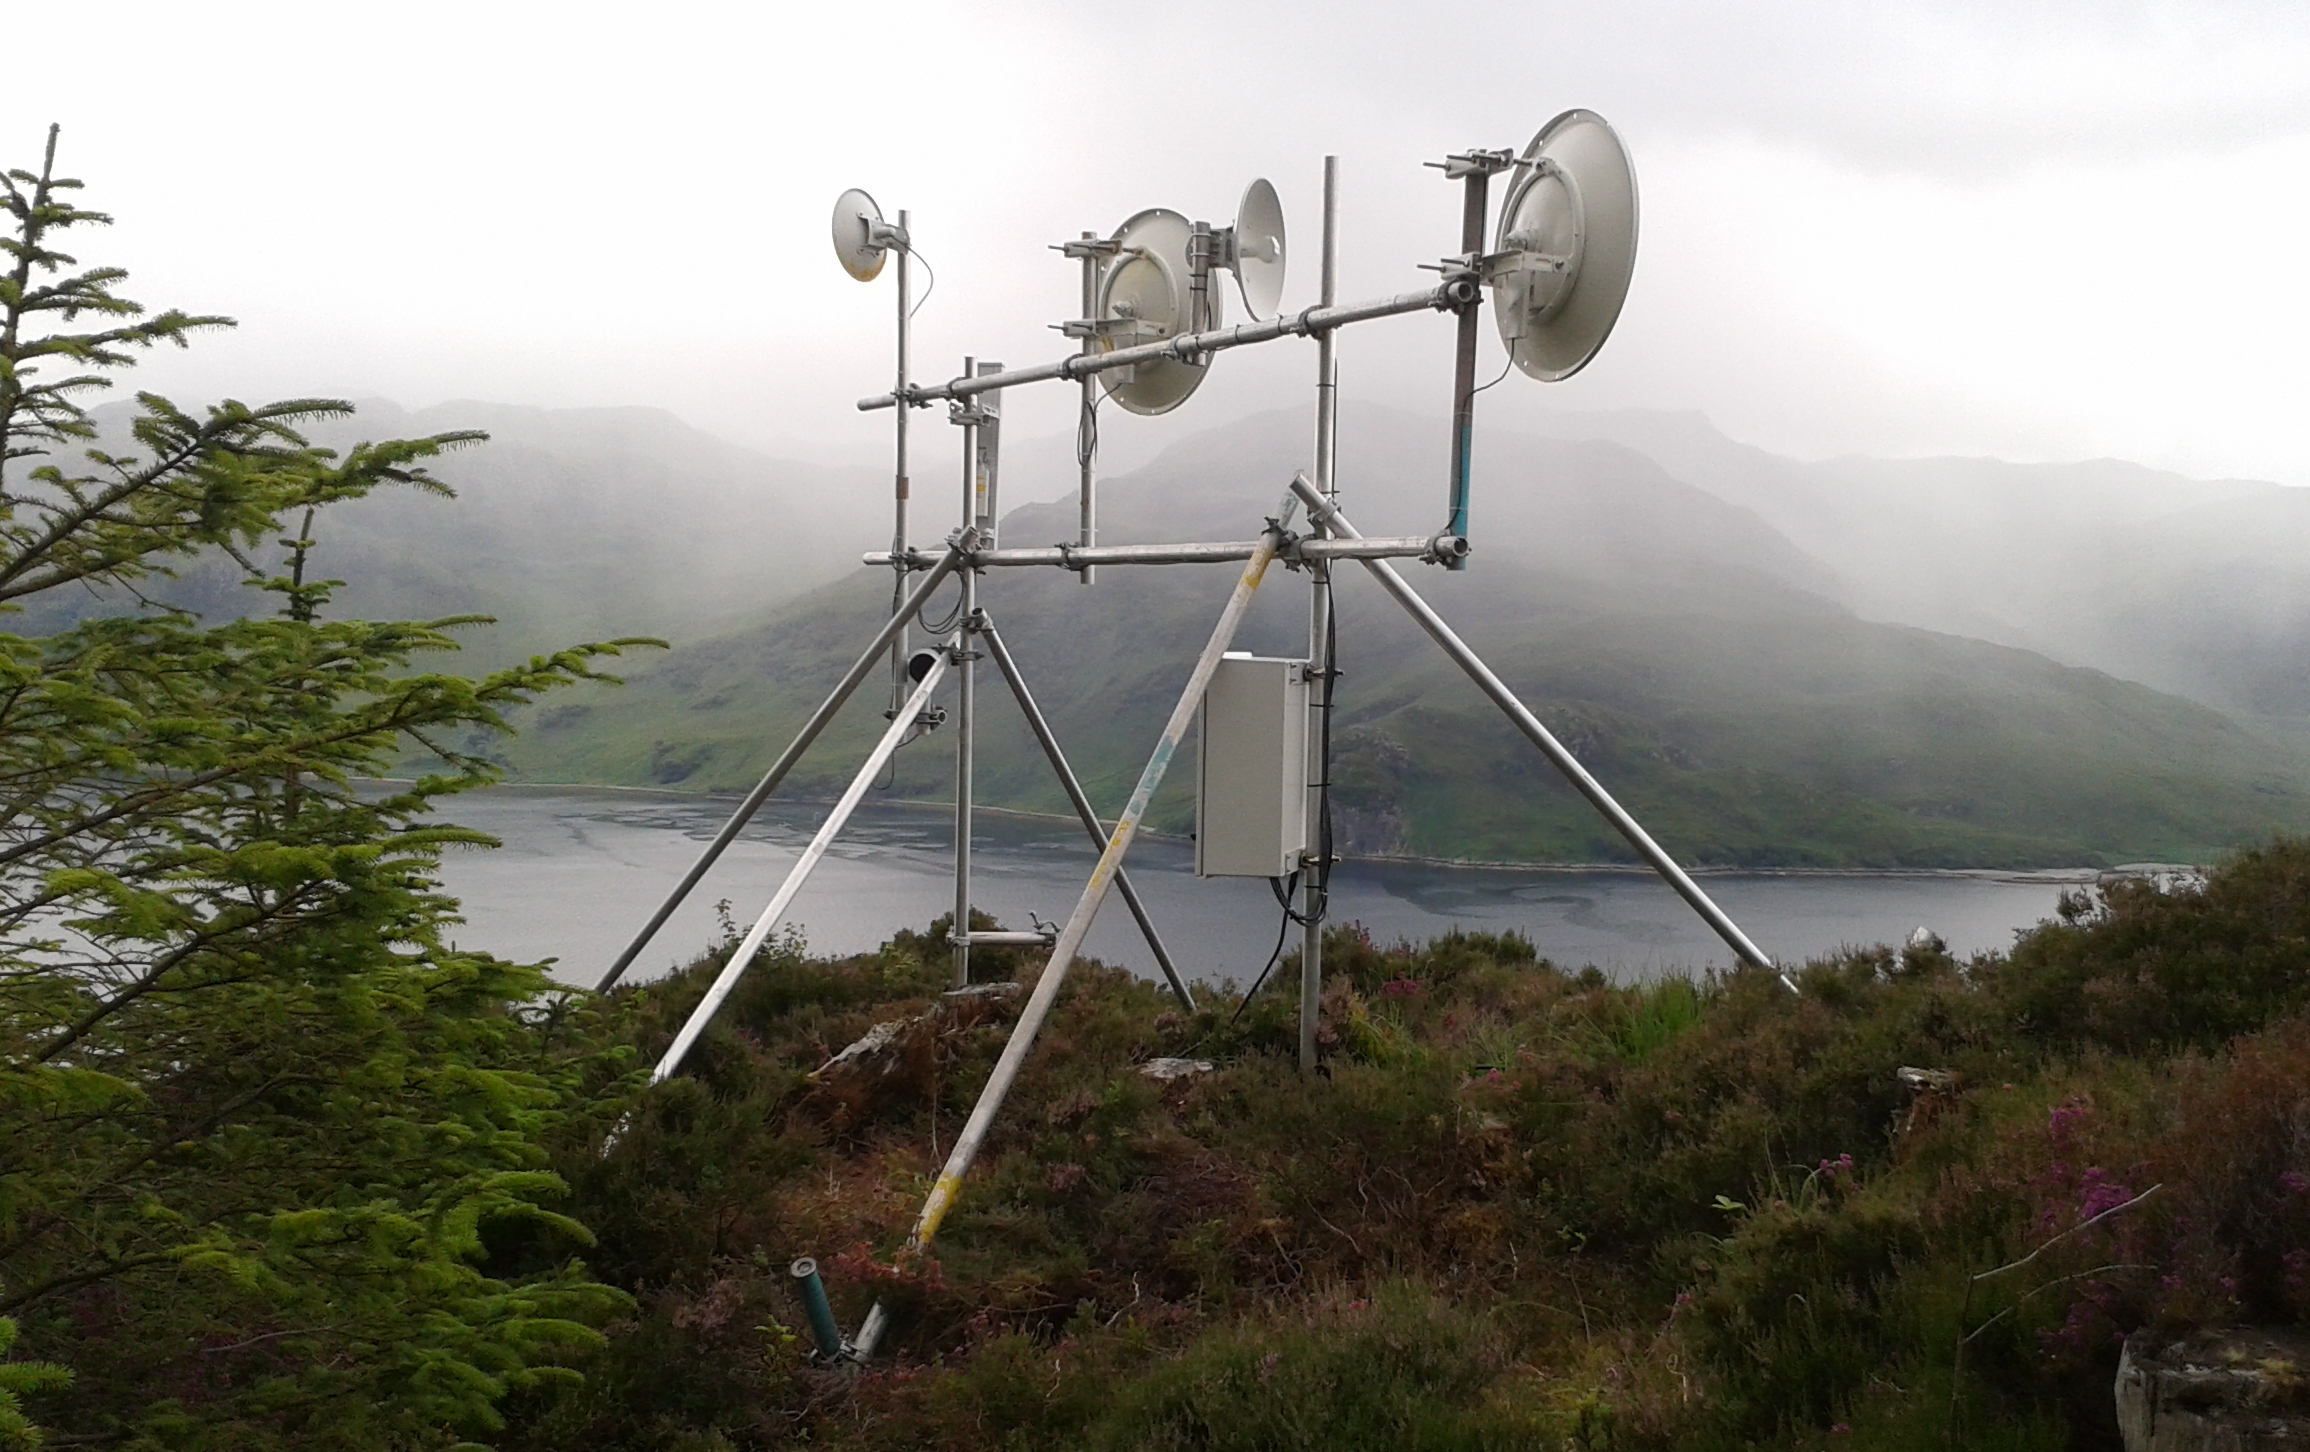
\includegraphics[width=\columnwidth]{figs/mhialairigh-from-behind}
 \caption{A basic relay}
\label{fig:mhialairigh}
\end{figure}

Recently, it has become possible to obtain adequate bandwidth at two major exchanges, but the cost is only reasonable if communities combine and buy at ``bulk'' prices.  For this one needs two things: an organization -- a co-operative -- that will act on behalf of the communities to obtain the economies of scale and a networking infrastructure

The terrain and the sociology of the Highlands and Island raises some important issues for both of these.
\begin{itemize}
\item The social communities do not always align well with the
  ``electronic'' communities. It is relatively easy to bounce signals
  back and forth across a loch or glen, but extremely hard to carry
  them over a 1000m high range of mountains. The reasons for this are
  social and economic and sometimes determined by the ways in which
  communities obtain funding.%\footnote{Knoydart is an isolated
    %% peninsula (see Fig.~\ref{fig:whixmap})  of which the North and
    %% West coasts are served by a network based on Loch Hourn and the
    %% South coast is served by Loch Nevis.  Contrast this with the Sleat
    %% peninsula which could, rationally,  be split into three sections,
    %% served by Loch Hourn, Loch Nevis and Eigg, but is run
    %% independently as a single entity with three connections to the
    %% rest of the world.}. 
\item Communities structure their networks in various ways, and the
  complexity varies from a single point-to multipoint distribution
  system to a network with six relays  eight or more point-to-point
  links.  In some cases the networks have more than one physical path
  between relays for redundancy. 
\item Many adjacent communities have successfully duplicated the local
  access network model. Together they cover a significantly large,
  contiguous geographical area.
\item Communities may temporarily share resources (links or backhaul)
  when appropriate but this is not done in a systematic or organised
  fashion.
\end{itemize}

%% Stimulated in part by developments in the Highlands and Islands,
%% communities in the Scottish Borders South of Edinburgh started to
%% develop similar networks.  While the terrain is also mountainous, the
%% communities are within 40km of Edinburgh where fibre services are
%% available.  However these are only affordable if the communities
%% combine to purchase bandwidth at scale. To this end a community
%% interest company, HUBS, was established whose members are the
%% communities itself.  In addition to backhaul, HUBS provides technical
%% help and other services.  It is anticipated that HUBS will extend its
%% reach to serve the West Coast and achieve further economies of scale,
%% for example in the puchase of transit.
